% (c) 2012-2013 Claudio Carboncini - claudio.carboncini@gmail.com
% (c) 2012-2014 Dimitrios Vrettos - d.vrettos@gmail.com

\chapter{Equazioni}

\section{Equazioni di grado superiore al primo riducibili al primo grado}

Nel capitolo \ref{cap:equazioni_I_grado} abbiamo affrontato le equazioni di primo grado. Adesso consideriamo le equazioni di grado superiore al primo che possono essere ricondotte ad equazioni di primo grado,
utilizzando la legge di annullamento del prodotto (legge \ref{legge:annullamento_del_prodotto} a pagina \pageref{legge:annullamento_del_prodotto}).

\begin{exrig}
 \begin{esempio}
Risolvere~$x^{2}-4=0$.

Il polinomio al primo membro può essere scomposto in fattori:~$(x-2)(x+2)=0$.
Per la legge di annullamento, il prodotto dei due binomi si annulla se~$x-2=0$ oppure se~$x+2=0$.
Di conseguenza si avranno le soluzioni:~$x=2$ e $x=-2$.
 \end{esempio}
\end{exrig}

In generale, se si ha un’equazione di grado~$n$ scritta in forma normale~$P(x)=0$ e se il polinomio~$P(x)$ è
fattorizzabile nel prodotto di~$n$ fattori di primo grado:
\begin{equation*}
(x-a_{1})(x-a_{2})(x-a_{3})\ldots (x-a_{n-1})(x-a_{n})=0
\end{equation*}
applicando la legge di annullamento del prodotto, le soluzioni dell’equazione si ottengono determinando le soluzioni delle singole~$n$
equazioni di primo grado, cioè risolvendo:
\begin{equation*}
x-a_{1}=0\text{,~~~}x-a_{2}=0\text{,~~~}x-a_{3}=0\text{,~~~}\ldots\text{,~~~}x-a_{n-1}=0\text{,~~~}x-a_{n}=0.
\end{equation*}
Pertanto l’insieme delle soluzioni dell’equazione data sarà:~$\IS=\{a_{1}\text{,~}a_{2}\text{,~}a_{3}\text{,~}\ldots\text{,~}a_{n-1}\text{,~}a_{n}\}$.

\begin{exrig}
 \begin{esempio}
Risolvere~$x^{2}-x-2=0$.

Scomponendo in fattori il polinomio al primo membro, ricercando quei due numeri la cui somma è pari a~$-1$ e il cui prodotto è pari a~$-2$, 
si ha:~$(x+1)(x-2)=0$.
Utilizzando la legge di annullamento del prodotto, si ottiene il seguente insieme di soluzioni:~$\IS=\{-1\text{,~}2\}$.
 \end{esempio}

 \begin{esempio}
Risolvere~$x^{4}-5x^{2}+4=0$.

Scomponendo in fattori il polinomio al primo membro, utilizzando la regola della scomposizione del particolare trinomio di secondo grado,
si ottiene:~$(x^{2}-1)(x^{2}-4)=0$. Scomponendo ulteriormente in fattori si ha:
\begin{equation*}
(x-1)(x+1)(x-2)(x+2)=0.
\end{equation*}
Per la legge di annullamento del prodotto è necessario risolvere le equazioni:
\begin{equation*}
x-1=0\: \Rightarrow\: x=1\text{,}\quad x+1=0\: \Rightarrow\: x=-1\text{,}\quad x-2=0\: \Rightarrow\: x=2\text{,}\quad x+2=0\: \Rightarrow\: x=-2.
\end{equation*}
L’insieme delle soluzioni:~$\IS=\{+1\text{,~}-1\text{,~}+2\text{,~}-2\}$.
 \end{esempio}

\end{exrig}

\ovalbox{\risolvii \ref{ese:20.1}, \ref{ese:20.2}, \ref{ese:20.3}, \ref{ese:20.4}, \ref{ese:20.5}, \ref{ese:20.6}, \ref{ese:20.7}, \ref{ese:20.8},
\ref{ese:20.9}, \ref{ese:20.10}}

\vspazio\ovalbox{\ref{ese:20.11}, \ref{ese:20.12}, \ref{ese:20.13}}

\section{Equazioni numeriche frazionarie}

Affrontiamo ora le equazioni in cui l'incognita compare anche al denominatore.

\begin{definizione} Un’equazione in cui l’incognita compare al denominatore si chiama \emph{frazionaria} o \emph{fratta}.
\end{definizione}

\begin{exrig}
 \begin{esempio}
Risolvere~$\dfrac{3x-2}{1+x}=\dfrac{3x}{x-2}$.
 \end{esempio}
Questa equazione si differenzia da quelle affrontate in precedenza per il fatto che l'incognita compare anche al denominatore.
Riflettendo sulla richiesta del problema, possiamo senz’altro affermare che, se esiste il valore che rende
la frazione al primo membro uguale alla frazione al secondo membro, esso non deve annullare nessuno dei due denominatori,
poiché in questo caso renderebbe priva di significato la scrittura, in quanto frazioni con denominatore~$0$ sono prive di significato.

Per risolvere un'equazione frazionaria, prima di tutto dobbiamo renderla nella forma
\begin{equation*}
\frac{F(x)}{G(x)}=0.
\end{equation*}

\begin{enumeratea}
 \item Determiniamo il~$\mcm$ dei denominatori, $\mcm=(1+x)\cdot (x-2)$.
    Osserviamo che per~$x = -1$ oppure per~$x = 2$ le frazioni perdono di significato, in quanto si annulla il denominatore;
 \item imponiamo le condizioni di esistenza:~$1+x\neq~0$ e~$x-2\neq~0$ cioè~$\CE x\neq -1\wedge x\neq~2$. La ricerca dei valori
    che risolvono l'equazione viene ristretta all'insieme~$\Dom=\insR-\{-1\text{,~}2\}$, detto \emph{dominio} dell’equazione o
    \emph{insieme di definizione};
 \item applichiamo il primo principio d’equivalenza trasportando al primo membro la frazione che si trova al secondo membro
    e riduciamo allo stesso denominatore ($\mcm$)
    \begin{equation*}
      \frac{(3x-2)\cdot (x-2)-3x\cdot (1+x)}{(1+x)\cdot (x-2)}=0;
    \end{equation*}
 \item applichiamo il secondo principio di equivalenza moltiplicando ambo i membri per il~$\mcm$,
    certamente diverso da zero per le condizioni poste precedentemente. L’equazione diventa:~$(3x-2)\cdot (x-2)-3x\cdot (1+x)=0$;
 \item eseguiamo le moltiplicazioni e sommiamo i monomi simili per portare l’equazione alla forma canonica:
    $3x^{2}-6x-2x+4-3x-3x^{2}=0\: \Rightarrow\: -11x=-4$;
 \item dividiamo ambo i membri per~$-11$, per il secondo principio di equivalenza si ha:~$x=\frac{4}{11}$;
 \item confrontiamo il valore trovato con le~$\CE$: in questo caso la soluzione appartiene al dominio~$\Dom$, quindi possiamo concludere
    che è accettabile. L’insieme soluzione è:~$\IS=\left\{\frac{4}{11}\right\}$.
\end{enumeratea}

%\newpage
 \begin{esempio}
Risolvere~$\dfrac{x^{2}+x-3}{x^{2}-x}=1-\dfrac{5}{2x}$.
\end{esempio}

\begin{enumeratea}
 \item Determiniamo il~$\mcm$ dei denominatori. Per fare questo dobbiamo prima scomporli in fattori.
    Riscriviamo:~$\dfrac{x^{2}+x-3}{x\cdot (x-1)}=1-\dfrac{5}{2x}$ con~$\mcm=2x\cdot (x-1)$;
 \item condizioni di esistenza: \[x-1\neq~0\wedge~2x\neq~0\text{,}\] cioè~$x\neq~1\wedge x\neq~0$. Il dominio è~$\Dom=\insR-\{1\text{,~}0\}$;
 \item trasportiamo al primo membro ed uguagliamo a zero \[\frac{x^{2}+x-3}{x\cdot (x-1)}-1+\frac{5}{2x}=0\]
    e riduciamo allo stesso denominatore ($\mcm$) ambo i membri \[\frac{2x^{2}+2x-6-2x^{2}+2x+5x-5}{2x\cdot (x-1)}=0;\]
 \item applichiamo il secondo principio di equivalenza moltiplicando ambo i membri per il~$\mcm$,
    certamente diverso da zero per le condizioni poste in precedenza. L’equazione diventa:~$2x^{2}+2x-6-2x^{2}+2x+5x-5=0$;
 \item riduciamo i monomi simili per portare l’equazione alla forma canonica:~$9x=11$;
 \item dividiamo ambo i membri per~$9$, otteniamo:~$x=\frac{11}{9}$;
 \item confrontando con le~$\CE$, la soluzione appartiene all’insieme~$\Dom$, dunque è accettabile e l’insieme soluzione è:
    $\IS=\left\{\frac{11}{9}\right\}$.
\end{enumeratea}

\end{exrig}

\ovalbox{\risolvii \ref{ese:20.15}, \ref{ese:20.16}, \ref{ese:20.17}, \ref{ese:20.18}, \ref{ese:20.19}, \ref{ese:20.20}, \ref{ese:20.21},
\ref{ese:20.22}, \ref{ese:20.23}, \ref{ese:20.24}, \ref{ese:20.25}}

\vspazio\ovalbox{\ref{ese:20.26}, \ref{ese:20.27}}

\section{Equazioni letterali}
Quando si risolvono problemi, ci si ritrova a dover tradurre nel linguaggio simbolico delle proposizioni del tipo:
<<Un lato di un triangolo scaleno ha lunghezza pari a~$k$ volte la lunghezza dell’altro e la loro somma è pari a~$2k$>>.
Poiché la lunghezza del lato del triangolo non è nota, ad essa si attribuisce il valore incognito~$x$ e quindi la proposizione
viene tradotta dalla seguente equazione:~$x+kx=2k$.

È possibile notare che i coefficienti dell’equazione non sono solamente numerici, ma contengono una lettera dell’alfabeto diversa
dall’incognita. Qual è il ruolo della lettera~$k$?
Essa prende il nome di \emph{parametro} ed è una costante che rappresenta dei numeri fissi, quindi, può assumere dei valori prefissati.
Ogni volta che viene fissato un valore di~$k$, l’equazione precedente assume una diversa forma. Infatti si ha:
\begin{center}
\begin{tabular}{cl}
\toprule
Valore di~$k$ & Equazione corrispondente\\
\midrule
$0$ & $x=0$\\
$2$ & $x+2x=4$\\
$-\frac{1}{2}$ & $x-\frac{1}{2}x=-1$\\
\bottomrule
\end{tabular}
\end{center}

Si può quindi dedurre che il parametro diventa una costante, all’interno dell’equazione nell’incognita~$x$, ogni volta che se ne sceglie il valore.

Si supponga che il parametro~$k$ assuma valori all’interno dell’insieme dei numeri reali. Lo scopo è quello di risolvere l’equazione,
facendo attenzione a rispettare le condizioni che permettono l’uso dei principi d’equivalenza e che permettono di ridurla in forma normale.

Riprendiamo l'equazione  $x+kx=2k$, raccogliamo a fattore comune la~$x$ si ha:
\begin{equation*}
 (k+1)x=2k.
\end{equation*}
Per determinare la soluzione di questa equazione di primo grado, è necessario utilizzare il secondo principio d’equivalenza e
dividere ambo i membri per il coefficiente~$k+1$.
Si ricordi però che il secondo principio ci permette di moltiplicare o dividere i due membri dell'equazione per una stessa espressione,
purché questa sia diversa da zero.
Per questa ragione, nella risoluzione dell’equazione~$(k+1)x=2k$ è necessario distinguere i due casi:
\begin{itemize*}
\item se~$k+1\neq~0$, cioè se~$k\neq -1$, è possibile dividere per~$k+1$ e si ha~$x=\dfrac{2k}{k+1}$;
\item se~$k+1=0$, cioè se~$k=-1$, sostituendo tale valore all'equazione si ottiene l’equazione~$(-1+1)x=2\cdot (-1)$,
   cioè~$0\cdot x=-2$ che risulta impossibile.
\end{itemize*}
Riassumendo si ha:
\begin{center}
\begin{tabular}{lcc}
\toprule
\multicolumn{3}{c} {$x+kx=2k$~~con~$k \in \insR$}\vspace{1.05ex}\\
Condizioni sul parametro & Soluzione & Equazione\\
\midrule
$k=-1$ & nessuna & impossibile \\
$k\neq-1$ & $x=\dfrac{2k}{k+1}$ & determinata \\
\bottomrule
\end{tabular}
\end{center}

Ritorniamo ora al problema sul triangolo, spesso nell’enunciato del problema sono presenti delle limitazioni implicite
che bisogna trovare. Infatti, dovendo essere~$x$ un lato del triangolo esso sarà un numero reale positivo.
Di conseguenza, dovendo essere l’altro lato uguale a~$k$ volte~$x$, il valore di~$k$ deve necessariamente essere anch'esso positivo, ovvero~$k>0$.
Di conseguenza il parametro~$k$ non può mai assumere il valore~$-1$ e quindi il problema geometrico ammette sempre una soluzione.

Questa analisi effettuata sui valori che può assumere il parametro~$k$, prende il nome di \emph{discussione dell’equazione}.
\begin{procedura}
Stabilire quando una equazione è determinata, indeterminata, impossibile.

In generale, data l'equazione~$ax+b=0$ si ha~$ax=-b$ e quindi:
\begin{enumeratea}
\item se~$a\neq~0$, l’equazione è determinata e ammette l’unica soluzione~$x=-\dfrac{b}{a}$;
\item se~$a=0$ e~$b\neq~0$, l’equazione è impossibile;
\item se~$a=0$ e~$b=0$, l’equazione è soddisfatta da tutti i valori reali di~$x$, ovvero è indeterminata.
\end{enumeratea}
\end{procedura}

\begin{exrig}
 \begin{esempio}
Risolvere e discutere~$1+x+m=(x+1)^{2}-x(x+m)$.

Dopo aver fatto i calcoli si ottiene l’equazione~$(m-1)\cdot x=-m$ e quindi si ha:
\begin{itemize*}
 \item Se~$m-1\neq~0$, cioè se~$m\neq~1$, è possibile dividere ambo i membri per~$m-1$ e si ottiene l’unica soluzione~$x=-{\dfrac{m}{m-1}}$;
 \item se~$m-1=0$, cioè se~$m=1$, sostituendo nell'equazione il valore~$1$ si ottiene~$0\cdot x=-1$, che risulta impossibile.
\end{itemize*}
 \end{esempio}

 \begin{esempio}
Risolvere e discutere~$(k+3)x=k+4x(k+1)$.

Effettuando i prodotti si ottiene l’equazione:~$(3k+1)x=-k$ e quindi si ha:
\begin{itemize*}
 \item Se~$3k+1\neq~0$, cioè se~$k\neq -{\frac{1}{3}}$, è possibile dividere ambo i membri per~$3k+1$ e si ottiene l’unica soluzione~$x=\dfrac{-k}{3k+1}$;
 \item se~$k=-{\frac{1}{3}}$, sostituendo questo valore di~$k$ nell'equazione si ottiene~$0\cdot x=\frac{1}{3}$, che risulta un'equazione impossibile.
\end{itemize*}
 \end{esempio}

 \begin{esempio}
Risolvere e discutere~$a^{2}\cdot x=a+1+x$.

Portiamo al primo membro tutti i monomi che contengono l'incognita~$a^{2}\cdot x-x=a+1$.
Raccogliamo a fattore comune l'incognita~$x\cdot \left(a^{2}-1\right)=a+1$.
Scomponendo in fattori si ha l'equazione~$x\cdot \left(a-1\right)\left(a+1\right)=a+1$.

I valori di~$a$ che annullano il coefficiente dell'incognita sono~$a=1$ e~$a=-1$.
\begin{itemize*}
 \item Se nell'equazione sostituisco~$a=1$, ottengo l'equazione~$0x=2$ che è impossibile;
 \item se sostituisco~$a=-1$, ottengo l'equazione~$0x=0$ che è indeterminata;
 \item escludendo i casi~$a=1$ e~$a=-1$, che annullano il coefficiente della~$x$, posso applicare il secondo principio
    di equivalenza delle equazioni e dividere primo e secondo membro per~$(a+1)(a-1)$, ottenendo~$x=\dfrac{a+1}{\left(a+1\right)\cdot \left(a-1\right)}=\dfrac{1}{a-1}$.
\end{itemize*}
 \end{esempio}
Ricapitolando:
se~$a=1$, allora~$\IS=\emptyset$; se~$a=-1$, allora~$\IS=\insR$; se~$a\neq +1\wedge a\neq -1$, allora~$\IS=\left\{\dfrac{1}{a-1}\right\}$.
\end{exrig}

\ovalbox{\risolvii \ref{ese:20.34}, \ref{ese:20.35}, \ref{ese:20.36}, \ref{ese:20.37}, \ref{ese:20.38}, \ref{ese:20.39}, \ref{ese:20.40}}

\subsection{Equazioni con due parametri}

\begin{exrig}
 \begin{esempio}
Risolvere e discutere~$(b+a)x-(b+2)(x+1)=-1$.

Mettiamo l'equazione in forma canonica:~$bx+ax-bx-b-2x-2=-1$.
Raccogliamo a fattore comune l'incognita~$(a-2)x=b+1$.
\begin{itemize*}
 \item Se~$a-2=0$ l'equazione è impossibile o indeterminata. In questo caso:
  \begin{itemize*}
   \item se~$b+1=0$ è indeterminata;
   \item se~$b+1\neq~0$ è impossibile;
  \end{itemize*}
 \item se~$a-2\neq~0$ l'equazione è determinata e la sua soluzione è~$x=\dfrac{b+1}{a-2}$.
\end{itemize*}
 \end{esempio}
Riassumendo:
se~$a=2\wedge b=-1$ allora~$\IS=\insR$; se~$a=2\wedge b\neq -1$ allora~$\IS=\emptyset$; se~$a\neq~2\wedge b\neq -1$ allora~$\IS=\left\{\dfrac{b+1}{a-2}\right\}$.
\end{exrig}

\ovalbox{\risolvii \ref{ese:20.41}, \ref{ese:20.42}, \ref{ese:20.43}}

\subsection{Equazioni letterali, caso in cui il denominatore contiene il parametro}

\begin{exrig}
 \begin{esempio}
Risolvere e discutere~$\dfrac{x+a}{2a-1}-\dfrac{1}{a-2a^{2}}=\dfrac{x}{a}$ con~$a\in \insR$.

Questa equazione è intera, pur presentando termini frazionari.
Sappiamo che ogni volta che viene fissato un valore per il parametro, l’equazione assume una forma diversa;
la presenza del parametro al denominatore ci obbliga ad escludere dall’insieme dei numeri reali quei valori che annullano il denominatore.

Per~$a=0\vee a=\frac{1}{2}$ si annullano i denominatori, quindi l’equazione è priva di significato.
Per risolvere l’equazione abbiamo bisogno delle condizioni di esistenza~$\CE a\neq~0$ e $a\neq \frac{1}{2}$.

Procediamo nella risoluzione, riduciamo allo stesso denominatore ambo i membri dell’equazione:
$\dfrac{a\cdot (x+a)+1}{a\cdot (2a-1)}=\dfrac{x\cdot (2a-1)}{a\cdot (2a-1)}$.
Applichiamo il secondo principio moltiplicando ambo i membri per il~$\mcm$, otteniamo:~$ax+a^{2}+1=2ax-x$
che in forma canonica è
\begin{equation*}
 x\cdot (a-1)=a^{2}+1.
\end{equation*}

Il coefficiente dell’incognita dipende dal valore assegnato al parametro $a$; procediamo quindi alla discussione:
\begin{itemize*}
 \item se~$a-1\neq~0$ cioè~$a\neq~1$ possiamo applicare il secondo principio e dividere ambo i membri per il coefficiente
    $a-1$ ottenendo~$x=\dfrac{a^{2}+1}{a-1}$. L’equazione è determinata:
    \[\IS=\left\{\frac{a^{2}+1}{a-1}\right\};\]
 \item se~$a-1=0$ cioè~$a=1$ l’equazione diventa~$0\cdot x=2$. L’equazione è impossibile:~$\IS=\emptyset$.
\end{itemize*}

Riassumendo si ha:
\begin{center}
\begin{tabular}{lll}
\toprule
\multicolumn{3}{c} {$\frac{x+a}{2a-1}-\frac{1}{a-2a^{2}}=\frac{x}{a}$~~con~$a\in \insR$}\vspace{1.05ex}\\
Condizioni sul parametro & Insieme Soluzione & Equazione\\
\midrule
$a=0\vee a=\frac{1}{2}$ & & priva di significato\\
$a=1$ & $\IS=\emptyset$ & impossibile \\
$a\neq~0\wedge a\neq \frac{1}{2}\wedge a\neq~1$ & $\IS=\left\{\frac{a^{2}+1}{a-1}\right\}$ & determinata \\
\bottomrule
\end{tabular}
\end{center}
 \end{esempio}

 \begin{esempio}
Risolvere e discutere~$\dfrac{a-x}{a-2}+\dfrac{2ax}{a^{2}-4}-\dfrac{2-x}{a+2}=0$ con~$a\in \insR$.

Scomponendo i denominatori troviamo il~$\mcm=a^2-4$.
Pertanto se~$a=2$ o~$a=-2$ il denominatore si annulla e quindi l’equazione è priva di significato.
Per poter procedere nella risoluzione poni le~$\CE a\neq -2\wedge a\neq~2$.

Riducendo allo stesso denominatore:~$\dfrac{(a-x)(a+2)+2ax-(2-x)(a-2)}{(a+2)(a-2)}=0$.

Applica il secondo principio per eliminare il denominatore e svolgi i calcoli. Arrivi alla forma canonica che è
 $2\cdot (a-2)\cdot x=a^{2}+4$.

Per le~$\CE$ sul parametro, il coefficiente dell’incognita è sempre diverso da zero, pertanto puoi dividere per~$2(a-2)$ e ottieni
$x=\dfrac{a^{2}+4}{2(a-2)}$.

Riassumendo si ha:
\begin{center}
\begin{tabular}{lll}
\toprule
\multicolumn{3}{c} {$\frac{a-x}{a-2}+\frac{2ax}{a^{2}-4}-\frac{2-x}{a+2}=0$ con~$a\in \insR$}\vspace{1.05ex}\\
Condizioni sul parametro & Insieme Soluzione & Equazione\\
\midrule
$a=-2\vee a=+2$ & & priva di significato\\
$a\neq -2\wedge a\neq +2$ & $\IS=\left\{\frac{a^{2}+4}{2(a-2)}\right\}$ & determinata \\
\bottomrule
\end{tabular}
\end{center}
 \end{esempio}
\end{exrig}

\subsection{Equazioni letterali frazionarie}

\subsubsection{Caso in cui il denominatore contiene solo l’incognita}

\begin{exrig}
 \begin{esempio}
Risolvere e discutere~$\dfrac{x+4a}{3x}=a-\dfrac{2x+2a}{6x}$ con~$a\in \insR$.

Questa equazione è frazionaria o fratta perché nel denominatore compare l’incognita.
Sappiamo che risolvere un’equazione significa determinare i valori che, sostituiti all’incognita, rendono vera
l’uguaglianza tra il primo e il secondo membro. Non sappiamo determinare tale valore solamente analizzando l’equazione,
ma certamente possiamo dire che non dovrà essere~$x = 0$ perché tale valore, annullando i denominatori, rende privi di
significato entrambi i membri dell’equazione.

Poniamo allora una condizione sull’incognita: la soluzione è accettabile se~$x\neq~0$.
Non abbiamo invece nessuna condizione sul parametro.

Procediamo quindi con la riduzione allo stesso denominatore di ambo i membri dell’equazione
$\dfrac{2x+8a}{6x}=\dfrac{6ax-2x-2a}{6x}$; eliminiamo il denominatore che per la condizione posta è diverso da zero.
Eseguiamo i calcoli al numeratore e otteniamo~$4x-6ax=-10a$ da cui la forma canonica:
\begin{equation*}
 x\cdot (3a-2)=5a.
\end{equation*}

Il coefficiente dell’incognita contiene il parametro, quindi procediamo alla discussione:
\begin{enumeratea}
 \item se~$3a-2\neq~0$ cioè~$a\neq \frac{2}{3}$ possiamo applicare il secondo principio e dividere ambo i membri per il coefficiente
      $3a-2$ ottenendo~$x=\frac{5a}{3a-2}$. L’equazione è determinata:~$\IS=\left\{\frac{5a}{3a-2}\right\}$.
      A questo punto dobbiamo ricordare la condizione sull'incognita, cioè~$x\neq~0$,
      quindi la soluzione è accettabile se~$x=\frac{5a}{3a-2}\neq~0 \Rightarrow a\neq~0$;
 \item se~$3a-2=0$ cioè~$a=\frac{2}{3}$ l’equazione diventa~$0\cdot x=\frac{10}{3}$, cioè l’equazione è impossibile:~$\IS=\emptyset$.
\end{enumeratea}
Riassumendo si ha la tabella:
\begin{center}
\begin{tabular}{llll}
\toprule
\multicolumn{4}{c} {$\dfrac{x+4a}{3x}=a-\dfrac{2x+2a}{6x}$ con~$a\in \insR$}\vspace{1.05ex}\\
\multicolumn{2}{c}{Condizioni} & &\\
parametro & incognita & Insieme Soluzione & Equazione\\
\midrule
 &$x\neq0$ & & \\
$a=\frac{2}{3}$ & & $\IS=\emptyset$ & impossibile \\
$a\neq\frac{2}{3}$ & & $\IS=\left\{\frac{5a}{3a-2}\right\}$ & determinata \\
$a\neq \frac{2}{3}\wedge a\neq0$ & accettabile &$x=\frac{5a}{3a-2}$ & \\
\bottomrule
\end{tabular}
\end{center}
 \end{esempio}
\end{exrig}

\subsubsection{Caso in cui il denominatore contiene sia il parametro che l’incognita}

\begin{exrig}
 \begin{esempio}
Risolvere e discutere~$\dfrac{2x+b}{x}+\dfrac{2x+1}{b-1}=\dfrac{2x^{2}+b^{2}+1}{bx-x}$ con~$b\in \insR$.
\end{esempio}
L’equazione è fratta; il suo denominatore contiene sia l’incognita $x$ che il parametro $b$.
Scomponiamo in fattori i denominatori
\[\frac{2x+b}{x}+\frac{2x+1}{b-1}=\frac{2x^{2}+b^{2}+1}{x\cdot (b-1)}.\]

Determiniamo le condizioni di esistenza che coinvolgono il parametro~$\CE b\neq~1$ e
le condizioni sull’incognita: soluzione accettabile se~$x\neq~0$.

Riduciamo allo stesso denominatore ed eliminiamolo in quanto per le condizioni poste è diverso da zero.
L'equazione canonica è~$x\cdot (2b-1)=b+1.$

Il coefficiente dell’incognita contiene il parametro quindi occorre fare la discussione:

\begin{enumeratea}
 \item se~$2b-1\neq~0$ cioè~$b\neq \frac{1}{2}$ possiamo dividere ambo i membri per~$2b-1$, otteniamo:
    $x=\frac{b+1}{2b-1}$. L’equazione è determinata, l'insieme delle soluzioni è~$\IS=\left\{\frac{b+1}{2b-1}\right\}$;
    la soluzione è accettabile se verifica la condizione di esistenza~$x\neq~0$ da cui si ha
    \[x=\frac{b+1}{2b-1}\neq~0\quad \Rightarrow\quad b\neq -1\text{,}\]
    cioè se~$b=-1$ l'equazione ha una soluzione che non è accettabile, pertanto è impossibile;
 \item se~$2b-1=0$ cioè~$b=\frac{1}{2}$ l’equazione diventa~$0\cdot x=\frac{3}{2}$. L’equazione è impossibile, l'insieme delle soluzioni è vuoto:
    $\IS=\emptyset$.
\end{enumeratea}

La tabella che segue riassume tutti i casi:
\begin{center}
\begin{tabular}{llll}
\toprule
\multicolumn{4}{c} {$\dfrac{2x+b}{x}+\dfrac{2x+1}{b-1}=\dfrac{2x^{2}+b^{2}+1}{bx-x}$ con~$b\in \insR$}\vspace{1.05ex}\\
\multicolumn{2}{c}{Condizioni} & &\\
parametro & incognita & Insieme Soluzione & Equazione\\
\midrule
$b=1$ & & & priva di significato\\
$b\neq1$ &$x\neq0$ & & \\
$b=\frac{1}{2}\vee b=-1$ & & $\IS=\emptyset$ & impossibile \\
$b\neq~1\wedge b\neq \frac{1}{2}$ & & $\IS=\left\{\frac{b+1}{2b-1}\right\}$ & determinata \\
$b\neq~1\wedge b\neq \frac{1}{2}\wedge b\neq -1$ & accettabile &$x=\frac{b+1}{2b-1}$ & \\
\bottomrule
\end{tabular}
\end{center}

\end{exrig}

\ovalbox{\risolvii \ref{ese:20.44}, \ref{ese:20.45}, \ref{ese:20.46}, \ref{ese:20.47}, \ref{ese:20.48}, \ref{ese:20.49}, \ref{ese:20.50}, \ref{ese:20.51}}

\section{Equazioni letterali e formule inverse}

Le formule di geometria, di matematica finanziaria e di fisica possono essere viste come equazioni letterali.
I due principi di equivalenza delle equazioni permettono di ricavare le cosiddette formule inverse, ossia di risolvere
un'equazione letterale rispetto a una delle qualsiasi lettere incognite che vi compaiono.
%\newpage
\begin{exrig}
 \begin{esempio}
Area del triangolo~$A=\dfrac{b\cdot h}{2}$.

Questa equazione è stata risolta rispetto all'incognita~$A$, ossia se sono note le misure della base~$b$ e dell'altezza~$h$
è possibile ottenere il valore dell'area~$A$.

È possibile risolvere l'equazione rispetto a un'altra lettera pensata come incognita.
Note le misure di~$A$ e di~$b$ ricaviamo~$h$. Per il primo principio di equivalenza moltiplichiamo per~$2$
entrambi i membri dell'equazione
\[A=\frac{b\cdot h}{2}\quad\Rightarrow\quad~2A=b\cdot h\]
dividiamo entrambi i membri per~$b$ ottenendo~$\frac{2A}{b}=h$.
Ora basta invertire primo e secondo membro: \[h=\frac{2A}{b}.\]
 \end{esempio}

 \begin{esempio}
Formula del montante~$M=C(1+it)$.

Depositando un capitale~$C$ per un periodo di tempo~$t$ (in anni), a un tasso di interesse annuo~$i$,
si ha diritto al montante~$M$.

Risolviamo l'equazione rispetto al tasso di interesse~$i$, ossia supponiamo di conoscere il capitale depositato~$C$, il montante~$M$
ricevuto alla fine del periodo~$t$ e ricaviamo il tasso di interesse che ci è stato applicato.
Partendo da~$M=C(1+it)$, dividiamo primo e secondo membro per~$C$, otteniamo \[\frac{M}{C}=1+it;\]
sottraiamo~$1$ al primo e al secondo membro, otteniamo
\[\frac{M}{C}-1=it;\] dividiamo primo e secondo membro per~$t$,
otteniamo
\[i=\frac{\left(\frac{M}{C}-1\right)}{t}\quad\Rightarrow\quad%
i=\frac{1}{t}\cdot \left(\frac{M}{C}-1\right)\quad\Rightarrow\quad i=\frac{M-C}{t\cdot C}.\]
 \end{esempio}

 \begin{esempio}
Formula del moto rettilineo uniforme~$s=s_{0}+v\cdot t$.

Un corpo in una posizione~$s_0$, viaggiando alla velocità costante~$v$, raggiunge dopo un intervallo di tempo~$t$ la posizione~$s$.

Calcoliamo~$v$ supponendo note le altre misure.
Partendo dalla formula~$s=s_{0}+v\cdot t$ sottraiamo ad ambo i membri~$s_0$, otteniamo~$s-s_{0}=v\cdot t$;
dividiamo primo e secondo membro per~$t$, otteniamo \[\frac{s-s_{0}}{t}=v.\]
 \end{esempio}

\end{exrig}

\ovalbox{\risolvii \ref{ese:20.53}, \ref{ese:20.54}, \ref{ese:20.55}, \ref{ese:20.56}, \ref{ese:20.57}, \ref{ese:20.58}, \ref{ese:20.59}, \ref{ese:20.60}, \ref{ese:20.61}}

\vspazio\ovalbox{\ref{ese:20.62}, \ref{ese:20.63}, \ref{ese:20.64}, \ref{ese:20.65}}

\newpage
% (c) 2012-2013 Claudio Carboncini - claudio.carboncini@gmail.com
% (c) 2012-2014 Dimitrios Vrettos - d.vrettos@gmail.com

\section{Esercizi}

\subsection{Esercizi dei singoli paragrafi}

\subsubsection*{\thechapter.1 - Equazioni di grado superiore al primo riducibili al primo grado}

\begin{esercizio}[\Ast]
\label{ese:20.1}
Risolvere le seguenti equazioni riconducendole a equazioni di primo grado.
\begin{multicols}{2}
\begin{enumeratea}
 \item $x^{2}+2x=0$;
 \item $x^{2}+2x-9x-18=0$;
 \item $2x^{2}-2x-4=0$;
 \item $4x^{2}+16x+16=0$.
\end{enumeratea}
\end{multicols}
\end{esercizio}

\begin{esercizio}[\Ast]
\label{ese:20.2}
Risolvere le seguenti equazioni riconducendole a equazioni di primo grado.
\begin{multicols}{2}
\begin{enumeratea}
 \item $x^{2}-3x-10=0$;
 \item $x^{2}+4x-12=0$;
 \item $3x^{2}-6x-9=0$;
 \item $x^{2}+5x-14=0$.
\end{enumeratea}
\end{multicols}
\end{esercizio}

\begin{esercizio}[\Ast]
\label{ese:20.3}
Risolvere le seguenti equazioni riconducendole a equazioni di primo grado.
\begin{multicols}{2}
\begin{enumeratea}
 \item $-3x^{2}-9x+30=0$;
 \item $-{\dfrac{3}{2}}x^{2}+\dfrac{3}{2}x+63=0$;
 \item $7x^{2}+14x-168=0$;
 \item $\dfrac{7}{2}x^{2}+7x-168=0$.
\end{enumeratea}
\end{multicols}
\end{esercizio}

\begin{esercizio}[\Ast]
\label{ese:20.4}
Risolvere le seguenti equazioni riconducendole a equazioni di primo grado.
\begin{multicols}{2}
\begin{enumeratea}
 \item $x^{4}-16x^{2}=0$;
 \item $2x^{3}+2x^{2}-20x+16=0$;
 \item $-2x^{3}+6x+4=0$;
 \item $-x^{6}+7x^{5}-10x^{4}=0$.
\end{enumeratea}
\end{multicols}
\end{esercizio}

\begin{esercizio}[\Ast]
\label{ese:20.5}
Risolvere le seguenti equazioni riconducendole a equazioni di primo grado.
\begin{multicols}{2}
\begin{enumeratea}
 \item $x^{3}-3x^{2}-13x+15=0$;
 \item $x^{2}+10x-24=0$;
 \item $2x^{3}-2x^{2}-24x=0$;
 \item $x^{4}-5x^{2}+4=0$.
\end{enumeratea}
\end{multicols}
\end{esercizio}

\begin{esercizio}[\Ast]
\label{ese:20.6}
Risolvere le seguenti equazioni riconducendole a equazioni di primo grado.
\begin{multicols}{2}
\begin{enumeratea}
 \item $-x^{3}-5x^{2}-x-5=0$;
 \item $\dfrac{3}{4}x^{3}-\dfrac{3}{4}x=0$;
 \item $-4x^{4}-28x^{3}+32x^{2}=0$;
 \item $-{\dfrac{6}{5}}x^{3}-\dfrac{6}{5}x^{2}+\dfrac{54}{5}x+\dfrac{54}{5}=0$.
\end{enumeratea}
\end{multicols}
\end{esercizio}

\begin{esercizio}[\Ast]
\label{ese:20.7}
Risolvere le seguenti equazioni riconducendole a equazioni di primo grado.
\begin{multicols}{2}
\begin{enumeratea}
 \item $-4x^{3}+20x^{2}+164x-180=0$;
 \item $5x^{3}+5x^{2}-80x-80=0$;
 \item $-3x^{3}+18x^{2}+3x-18=0$;
 \item $4x^{3}+8x^{2}-16x-32=0$.
\end{enumeratea}
\end{multicols}
\end{esercizio}

\begin{esercizio}[\Ast]
\label{ese:20.8}
Risolvere le seguenti equazioni riconducendole a equazioni di primo grado.
\begin{multicols}{2}
\begin{enumeratea}
 \item $x^{3}+11x^{2}+26x+16=0$;
 \item $2x^{3}+6x^{2}-32x-96=0$;
 \item $2x^{3}+16x^{2}-2x-16=0$;
 \item $-2x^{3}+14x^{2}-8x+56=0$.
\end{enumeratea}
\end{multicols}
\end{esercizio}
%\newpage
\begin{esercizio}[\Ast]
\label{ese:20.9}
Risolvere le seguenti equazioni riconducendole a equazioni di primo grado.
\begin{multicols}{2}
\begin{enumeratea}
 \item $2x^{3}+12x^{2}+18x+108=0$;
 \item $x^{4}-10x^{3}+35x^{2}-50x+24=0$;
 \item $-2x^{3}-12x^{2}+18x+28=0$;
 \item $-5x^{4}+125x^{2}+10x^{3}-10x-120=0$.
\end{enumeratea}
\end{multicols}
\end{esercizio}

\begin{esercizio}[\Ast]
\label{ese:20.10}
Risolvere le seguenti equazioni riconducendole a equazioni di primo grado.
\begin{multicols}{2}
\begin{enumeratea}
 \item $\dfrac{7}{6}x^{4}-\dfrac{161}{6}x^{2}-21x+\dfrac{140}{3}=0$;
 \item $(x^{2}-6x+8)(x^{5}-3x^{4}+2x^{3})=0$;
 \item $\left(25-4x^{2}\right)^{4}\left(3x-2\right)^{2}=0$;
 \item $(x-4)^{3}\left(2x^{3}-4x^{2}-8x+16\right)^{9}=0$.
\end{enumeratea}
\end{multicols}
\end{esercizio}

\begin{esercizio}[\Ast]
\label{ese:20.11}
Risolvere le seguenti equazioni riconducendole a equazioni di primo grado.
\begin{multicols}{2}
\begin{enumeratea}
 \item $(x^{3}-x)(x^{5}-9x^{3})(x^{2}+25)=0$;
 \item $x^{5}+3x^{4}-11x^{3}-27x^{2}+10x+24=0$;
 \item $2x^{2}-x-1=0$;
 \item $3x^{2}+5x-2=0$.
\end{enumeratea}
\end{multicols}
\end{esercizio}

\begin{esercizio}[\Ast]
\label{ese:20.12}
Risolvere le seguenti equazioni riconducendole a equazioni di primo grado.
\begin{multicols}{2}
\begin{enumeratea}
 \item $6x^{2}+x-2=0$;
 \item $2x^{3}-x^{2}-2x+1=0$;
 \item $3x^{3}-x^{2}-8x-4=0$;
 \item $8x^{3}+6x^{2}-5x-3=0$.
\end{enumeratea}
\end{multicols}
\end{esercizio}

\begin{esercizio}[\Ast]
\label{ese:20.13}
Risolvere le seguenti equazioni riconducendole a equazioni di primo grado.
\begin{multicols}{2}
\begin{enumeratea}
 \item $6x^{3}+x^{2}-10x+3=0$;
 \item $4x^{4}-8x^{3}-13x^{2}+2x+3=0$;
 \item $8x^{4}-10x^{3}-29x^{2}+40x-12=0$;
 \item $-12x^{3}+68x^{2}-41x+5=0$.
\end{enumeratea}
\end{multicols}
\end{esercizio}

\begin{esercizio}[\Ast]
\label{ese:20.14}
Risolvere la seguente equazione riconducendola a una equazione di primo grado.

$(x^{4}+3x^{3}-3x^{2}-11x-6)(4x^{6}-216x^{3}+2916)=0$;
\end{esercizio}

\subsubsection*{\thechapter.2 - Equazioni numeriche frazionarie}

\begin{esercizio}[\Ast]
\label{ese:20.15}
Risolvi le seguenti equazioni frazionarie.
\begin{multicols}{2}
\begin{enumeratea}
 \item $\dfrac{2}{x+1}=\dfrac{1}{x+2}$;
 \item $\dfrac{1}{x-1}=2$;
 \item $1-\dfrac{1}{x+1}=0$;
 \item $\dfrac{2x-4}{x-2}=0$.
\end{enumeratea}
\end{multicols}
\end{esercizio}

\begin{esercizio}[\Ast]
\label{ese:20.16}
Risolvi le seguenti equazioni frazionarie.
\begin{multicols}{2}
\begin{enumeratea}
 \item $\dfrac{x}{x+1}-\dfrac{1}{x-1}=1$;
 \item $\dfrac{1}{x-3}=\dfrac{x}{3-x}$;
 \item $\dfrac{x-1}{x^{2}-4}=-{\dfrac{5}{x+2}}$;
 \item $\dfrac{3}{x+1}=\dfrac{2}{x+1}$.
\end{enumeratea}
\end{multicols}
\end{esercizio}
%\newpage
\begin{esercizio}[\Ast]
\label{ese:20.17}
Risolvi le seguenti equazioni frazionarie.
\begin{multicols}{2}
\begin{enumeratea}
 \item $\dfrac{1}{3-x}-\dfrac{4}{2x-6}=0$;
 \item $\dfrac{x^{2}-1}{x-1}-1=2x+1$;
 \item $\dfrac{x}{x^{2}-4}=\dfrac{1}{x+2}$;
 \item $\dfrac{1}{x}-\dfrac{3}{x^{2}}=\dfrac{2-2x}{x^{3}}$.
\end{enumeratea}
\end{multicols}
\end{esercizio}

\begin{esercizio}[\Ast]
\label{ese:20.18}
Risolvi le seguenti equazioni frazionarie.
\begin{multicols}{2}
\begin{enumeratea}
 \item $\dfrac{x-2}{x-1}=\dfrac{x-1}{x-2}$;
 \item $\dfrac{x+3}{x+1}=x+3$;
 \item $\dfrac{3x+1}{3x^{2}+x}=1$;
 \item $\dfrac{6+x}{x-3}=\dfrac{x^{2}}{x-3}$.
\end{enumeratea}
\end{multicols}
\end{esercizio}

\begin{esercizio}[\Ast]
\label{ese:20.19}
Risolvi le seguenti equazioni frazionarie.
\begin{multicols}{2}
\begin{enumeratea}
 \item $\dfrac{1}{x-2}+\dfrac{2}{x+1}=\dfrac{3}{x^{2}-x-2}$;
 \item $\dfrac{5}{x-2}-\dfrac{6}{x+1}=\dfrac{3x-1}{x^{2}-x-2}$;
 \item $\dfrac{1}{1-x}-\dfrac{x}{x-1}=0$;
 \item $\dfrac{x+1}{x-1}-\dfrac{x}{1+x}=0$.
\end{enumeratea}
\end{multicols}
\end{esercizio}

\begin{esercizio}[\Ast]
\label{ese:20.20}
Risolvi le seguenti equazioni frazionarie.
\begin{multicols}{2}
\begin{enumeratea}
 \item $\dfrac{2x+1}{2x-1}+\dfrac{4x^{2}+1}{4x^{2}-1}=2$;
 \item $\dfrac{1}{x-1}+\dfrac{2}{x}+\dfrac{1}{x^{2}-x}=0$;
 \item $\dfrac{x-1}{x^{2}-2x+1}=\dfrac{2}{2-2x}$;
 \item $4-x^{2}=\dfrac{x^{2}+5x+6}{x+2}-1$.
\end{enumeratea}
\end{multicols}
\end{esercizio}

\begin{esercizio}[\Ast]
\label{ese:20.21}
Risolvi le seguenti equazioni frazionarie.
\begin{multicols}{2}
\begin{enumeratea}
 \item $\dfrac{5}{5x+1}+\dfrac{2}{2x-1}=\dfrac{1}{1-2x}$;
 \item $\dfrac{1}{x-2}+\dfrac{2}{x+1}=\dfrac{3}{x^{2}-x-2}$;
 \item $\dfrac{30}{x^{2}-25}+\dfrac{3}{5-x}=0$;
 \item $1+\dfrac{x-1}{x+1}=\dfrac{1}{x-2}+\dfrac{1-x^{2}}{x^{2}-x-2}$.
\end{enumeratea}
\end{multicols}
\end{esercizio}

\begin{esercizio}[\Ast]
\label{ese:20.22}
Risolvi le seguenti equazioni frazionarie.
\begin{multicols}{2}
\begin{enumeratea}
 \item $-{\dfrac{3x}{6-2x}}+\dfrac{5x}{10-5x}=\dfrac{1-x}{4-2x}$;
 \item $\dfrac{18x^{2}-9x-45}{4-36x^{2}}-\dfrac{6x+1}{9x-3}+\dfrac{21x-1}{18x+6}=0$;
 \item $\dfrac{1}{x+3}-\dfrac{1}{2-x}=\dfrac{x+3}{x^{2}+x-6}$;
 \item $\dfrac{1+2x}{1-2x}+\dfrac{1-2x}{1+2x}=\dfrac{6-8x^{2}}{1-4x^{2}}$.
\end{enumeratea}
\end{multicols}
\end{esercizio}

\begin{esercizio}[\Ast]
\label{ese:20.23}
Risolvi le seguenti equazioni frazionarie.
\begin{multicols}{2}
\begin{enumeratea}
 \item $\dfrac{3x}{x-2}+\dfrac{6x}{x^{2}-4x+4}=\dfrac{3x^{2}}{(x-2)^{2}}$;
 \item $(4x+6)\left(\dfrac{4}{x+1}-\dfrac{1}{x-1}\right)=0$;
 \item $\dfrac{5x}{3x^{2}-18x+15}-\dfrac{2}{3x-3}=\dfrac{5}{18x-90}$;
 \item $(x-4)(x+3)=\dfrac{(x-4)(x+3)}{x-2}$.
\end{enumeratea}
\end{multicols}
\end{esercizio}
%\newpage
\begin{esercizio}[\Ast]
\label{ese:20.24}
Risolvi le seguenti equazioni frazionarie.
\begin{multicols}{2}
\begin{enumeratea}
 \item $\dfrac{1}{3x+2}-\dfrac{3}{2-x}=\dfrac{10x+4}{3x^{2}-4x-4}$;
 \item $\dfrac{2x+1}{x+3}+\dfrac{1}{x-4}=\dfrac{4x-9}{x^{2}-x-12}$;
 \item $\dfrac{1}{x-1}-\dfrac{1}{x}=\dfrac{(x+1)^{2}}{2(x^{2}-1)}+1$;
 \item $\dfrac{x^{2}-1}{x+1}-\dfrac{1}{x+2}=\dfrac{x+1}{x+2}-x$.
\end{enumeratea}
\end{multicols}
\end{esercizio}

\begin{esercizio}[\Ast]
\label{ese:20.25}
Risolvi le seguenti equazioni frazionarie.
\begin{multicols}{2}
\begin{enumeratea}
 \item $\dfrac{1}{x+3}-\dfrac{2}{x+2}=\dfrac{3x-6}{x^{2}+5x+6}$;
 \item $\dfrac{2x-3}{x+2}+\dfrac{1}{x-4}=\dfrac{2}{x^{2}-2x-8}$;
 \item $\dfrac{x-1}{x+2}-\dfrac{x+2}{x-1}=\dfrac{1}{x^{2}+x-2}$;
 \item $\dfrac{3}{x-1}+\dfrac{1}{x+1}=\dfrac{12-x}{x^{2}-1}$.
\end{enumeratea}
\end{multicols}
\end{esercizio}

\begin{esercizio}[\Ast]
\label{ese:20.26}
Risolvi le seguenti equazioni frazionarie.
\begin{multicols}{2}
\begin{enumeratea}
 \item $\dfrac{1}{2} \left(x-\dfrac{1}{x}\right)-2\left(1-\dfrac{1}{x}\right)=\dfrac{x^{2}-1}{x}$;
 \item $\left(40-10x^{2}\right)^{3} \left(\dfrac{3x-1}{x+2}-\dfrac{3x}{x+1}\right)=0$;
 \item $\dfrac{x}{2x+1}+\dfrac{x+1}{2(x+2)}=\dfrac{x-1}{2x^{2}+5x+2}$;
 \item $\dfrac{3x+1}{x^{2}-9}+\dfrac{2}{3x^{2}-9x}=\dfrac{3}{x+3}$.
\end{enumeratea}
\end{multicols}
\end{esercizio}

\begin{esercizio}[\Ast]
\label{ese:20.27}
Risolvi le seguenti equazioni frazionarie.
\begin{multicols}{2}
\begin{enumeratea}
 \item $\dfrac{3(2x-3)}{x^{3}+27}+\dfrac{1}{x+3}=\dfrac{x}{x^{2}-3x+9}$;
 \item $\dfrac{1}{x^{2}-3x+2}+\dfrac{2}{x-1}=0$;
 \item $\dfrac{2x-1}{3x^{2}-75}-\dfrac{3-x}{x+5}+\dfrac{x-3}{10-2x}=\dfrac{7}{25-x^{2}}$;
 \item $\dfrac{x+2}{(x-3)^{2}}-\dfrac{1}{x-3}=\dfrac{4}{9-3x}$.
\end{enumeratea}
\end{multicols}
\end{esercizio}

\begin{esercizio}[\Ast]
\label{ese:20.28}
Risolvi le seguenti equazioni frazionarie.
\begin{enumeratea}
 \item $\left(\dfrac{1}{x+5}-\dfrac{1}{5}\right):\left(\dfrac{1}{x-5}+\dfrac{1}{5}\right)+\dfrac{x^{2}}{x^{2}-5x}=0$;
 \item $\dfrac{1+2x}{x^{2}+2x}+\dfrac{x^{3}-6x+1}{x^{2}-4}=\dfrac{x^{2}-2x}{x-2}+\dfrac{1}{x^{2}-2x}$.
 \item $\left(1-\dfrac{1}{2}x\right):\left(1+\dfrac{1}{2}x\right)=\dfrac{2x+1}{6x+3}-\dfrac{1}{2}x+\dfrac{x^{2}}{2x+4}$;
 \item $\dfrac{3x-1}{1-2x}+\dfrac{x}{2x-1}-\dfrac{x^{3}-8}{x^{2}-4}:\dfrac{x^{2}+2x+4}{x^{2}+2x+1}=\dfrac{2-3x}{2x-6}\cdot {\dfrac{x^{2}-9}{4-9x^{2}}}-\dfrac{6x+7}{6}$;
 \item $\dfrac{2x}{6x-3}+\dfrac{x}{4-8x}+\left(\dfrac{1}{2x+1}-\dfrac{1}{2x-1}\right)\cdot {\dfrac{2x\left(x^{2}-1\right)}{8x^{2}-4x}}=\dfrac{x^{2}(5x-3)}{3(2x+1)(2x-1)^{2}}$;
 \item $\dfrac{3x^{2}-2x+3}{x^{2}-3x}+\dfrac{x+2}{3-x}=\left(\dfrac{x+1}{x}-1\right)\left(\dfrac{x^{2}}{x^{3}-27}+\dfrac{x}{x-3}\right):\dfrac{3x}{3x^{3}-81}+\dfrac{x^{2}-x+2}{3-x}$.
\end{enumeratea}
\end{esercizio}

\begin{esercizio}
\label{ese:20.29}
$\left(2x-4x^{2}+7\right)^{6}=-{\dfrac{1}{\left(x^{2}-5x+7\right)^{4}}}$. Osservando i due membri dell'equazione, senza svolgere i calcoli, puoi subito affermare che non esiste alcun numero reale che rende
vera l'uguaglianza?
\end{esercizio}

\begin{esercizio}[\Ast]
\label{ese:20.30}
Quale numero occorre aggiungere a numeratore e denominatore della frazione tre settimi perchè essa raddoppi di valore?
\end{esercizio}

\begin{esercizio}[\Ast]
\label{ese:20.31}
Quale numero occorre aggiungere a numeratore e denominatore della frazione due settimi perchè essa triplichi di valore?
\end{esercizio}

\begin{esercizio}
\label{ese:20.32}
Due amici A e B partono con le loro automobili nello stesso istante da due località diverse; A fa un viaggio di
$100\unit{km}$ a una certa velocità, B fa un viaggio di~$132\unit{km}$ ad una velocità che supera quella dell’amico di~$20\unit{km/h}$.
I due amici arrivano nello stesso istante all’appuntamento. Qual è la velocità di A?
\begin{center}
 % (c) 2012 Dimitrios Vrettos - d.vrettos@gmail.com
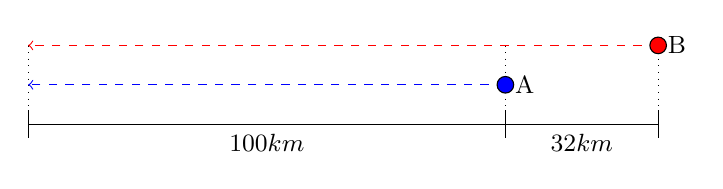
\begin{tikzpicture}[font=\small,x=10mm, y=10mm]
\draw (0,0) -- (8,0);
\foreach \x in {0,6.06,8}{
\draw (\x,5pt) -- (\x,-5pt);
\draw[dotted] (\x,1) -- (\x,0);
}

\draw[dashed, red, ->] (8,1) -- (0,1);
\draw[dashed, blue, ->] (6.06,.5) -- (0,.5);

\draw[fill=blue] (6.06,.5) circle (3pt) node [right] () {A};
\draw[fill=red] (8,1) circle (3pt) node [right] () {B};

\node[below] at (3.03,0) {$100\unit{km}$};
\node[below] at (7.03,0) {$32\unit{km}$};
\end{tikzpicture}
\end{center}
Traccia di soluzione:
\begin{itemize}
 \item se A e B partono insieme e arrivano insieme significa che hanno impiegato lo stesso tempo per fare il proprio viaggio;
 \item il tempo è dato dal rapporto tra lo spazio percorso e la velocità;
 \item la velocità di A è l’incognita del problema: la indichiamo con~$x$;
 \item l’equazione risolvente è~$\dfrac{110}{x}=\dfrac{132}{x+20}$.
\end{itemize}
Prosegui nella risoluzione.
\end{esercizio}

\begin{esercizio}
\label{ese:20.33}
Per percorrere~$480\unit{km}$ un treno impiega~$3$ ore di più di quanto impiegherebbe un aereo a percorrere~$\np[km]{1920}$.
L’aereo viaggia ad una velocità media che è~$8$ volte quella del treno. Qual è la velocità del treno?
\end{esercizio}

\subsubsection*{\thechapter.3 - Equazioni letterali}

\begin{esercizio}[\Ast]
\label{ese:20.34}
Risolvi e discuti le seguenti equazioni letterali nell'incognita~$x$.
\begin{multicols}{2}
\begin{enumeratea}
 \item $1+2x=a+1-2x$;
 \item $2x-\dfrac{7}{2}=ax-5$;
 \item $b^{2}x=2b+bx$;
 \item $ax+2=x+3$.
\end{enumeratea}
\end{multicols}
\end{esercizio}

\begin{esercizio}[\Ast]
\label{ese:20.35}
Risolvi e discuti le seguenti equazioni letterali nell'incognita~$x$.
\begin{multicols}{2}
\begin{enumeratea}
 \item $k(x+2)=k+2$;
 \item $(b+1)(x+1)=0$;
 \item $k^{2}x+2k=x+2$;
 \item $(a-1)(x+1)=x+1$.
\end{enumeratea}
\end{multicols}
\end{esercizio}

\begin{esercizio}
\label{ese:20.36}
Risolvi e discuti le seguenti equazioni letterali nell'incognita~$x$.
\begin{multicols}{2}
\begin{enumeratea}
 \item $ax+x-2a^{2}-2ax=0$;
 \item $3ax-2a=x\cdot (1-2a)+a\cdot (x-1)$;
 \item $x (3-5a)+2 (a-1)=(a-1) (a+1)$;
 \item $x+2a\cdot (x-2a)+1=0$.
\end{enumeratea}
\end{multicols}
\end{esercizio}
%\newpage
\begin{esercizio}[\Ast]
\label{ese:20.37}
Risolvi e discuti le seguenti equazioni letterali nell'incognita~$x$.
\begin{multicols}{2}
\begin{enumeratea}
 \item $(a-1)(x+1)=a-1$;
 \item $2k(x+1)-2=k(x+2)$;
 \item $a(a-1)x=2a(x-5)$;
 \item $3ax+a=2a^{2}-3a$.
\end{enumeratea}
\end{multicols}
\end{esercizio}

\begin{esercizio}[\Ast]
\label{ese:20.38}
Risolvi e discuti le seguenti equazioni letterali nell'incognita~$x$.
\begin{multicols}{2}
\begin{enumeratea}
 \item $3x-a=a(x-3)+6$;
 \item $2+2x=3ax+a-a^{2}x$;
 \item $x(a^{2}-4)=a+2$;
 \item $(x-m)(x+m)=(x+1)(x-1)$.
\end{enumeratea}
\end{multicols}
\end{esercizio}

\begin{esercizio}[\Ast]
\label{ese:20.39}
Risolvi e discuti le seguenti equazioni letterali nell'incognita~$x$.
\begin{multicols}{2}
\begin{enumeratea}
 \item $(a-2)^{2}x+(a-2)x+a-2=0$;
 \item $\left(9a^{2}-4\right)x=2(x+1)$;
 \item $(a-1)x=a^{2}-1$;
 \item $(a+2)x=a^{2}+a-1$.
\end{enumeratea}
\end{multicols}
\end{esercizio}

\begin{esercizio}[\Ast]
\label{ese:20.40}
Risolvi e discuti le seguenti equazioni letterali nell'incognita~$x$.
\begin{multicols}{2}
\begin{enumeratea}
 \item $a(x-1)^{2}=a(x^{2}-1)+2a$;
 \item $a^{3}x-a^{2}-4ax+4=0$;
 \item $bx\left(b^{2}+1\right)-(bx-1)\left(b^{2}-1\right)=2b^{2}$;
 \item $a(a-5)x+a(a+1)=-6(x-1)$:
 \item $(x+a)^{2}-(x-a)^{2}+(a-4)(a+4)=a^{2}$;
 \item $b(b+3)+x\left(6-b^{2}\right)=bx$.
\end{enumeratea}
\end{multicols}
\end{esercizio}

\begin{esercizio}[\Ast]
\label{ese:20.41}
Risolvi e discuti le seguenti equazioni nell'incognita~$x$ con due parametri.
\begin{multicols}{2}
\begin{enumeratea}
 \item $(m+1)(n-2)x=0$;
 \item $m(x-1)=n$;
 \item $(a+1)(b+1)x=0$;
 \item $(m+n)(x-1)=m-n$.
\end{enumeratea}
\end{multicols}
\end{esercizio}

\begin{esercizio}[\Ast]
\label{ese:20.42}
Risolvi e discuti le seguenti equazioni nell'incognita~$x$ con due parametri.
\begin{multicols}{2}
\begin{enumeratea}
 \item $x(2a-1)+2b(x-2)=-4a-x$;
 \item $ax-3+b=2(x+b)$;
 \item $(a+1)x=b+1$;
 \item $(a+b)(x-2)+3a-2b=2b(x-1)$.
\end{enumeratea}
\end{multicols}
\end{esercizio}

\begin{esercizio}[\Ast]
\label{ese:20.43}
Risolvi e discuti le seguenti equazioni nell'incognita~$x$ con due parametri.
\begin{enumeratea}
 \item $x(x+2)+3ax=b+x^{2}$;
 \item $(x-a)^{2}+b(2b+1)=(x-2a)^{2}+b-3a^{2}$.
\end{enumeratea}
\end{esercizio}

\begin{esercizio}[\Ast]
\label{ese:20.44}
Risolvi e discuti le seguenti equazioni che presentano il parametro al denominatore.
\begin{multicols}{2}
\begin{enumeratea}
 \item $\dfrac{x+2}{6a}+\dfrac{x-1}{2a^{2}}=\dfrac{1}{3a}$;
 \item $\dfrac{x-1}{b}+\dfrac{2x+3}{4b}=\dfrac{x}{4}$;
 \item $\dfrac{2x-1}{3a}+\dfrac{x}{3}=\dfrac{2}{a}$;
 \item $\dfrac{x}{a}+\dfrac{2x}{2-a}=\dfrac{a-x+2}{2a-a^{2}}$.
\end{enumeratea}
\end{multicols}
\end{esercizio}

\begin{esercizio}[\Ast]
\label{ese:20.45}
Risolvi e discuti le seguenti equazioni che presentano il parametro al denominatore.
\begin{multicols}{2}
\begin{enumeratea}
 \item $\dfrac{x}{a-1}+8=4a-\dfrac{x}{a-3}$;
 \item $\dfrac{x-1}{a-1}+\dfrac{x+a}{a}=\dfrac{a-1}{a}$;
 \item $\dfrac{a^{2}-9}{a+2}x=a-3$;
 \item $\dfrac{x+2}{a^{2}-2a}+\dfrac{x}{a^{2}+2a}+\dfrac{1}{a}=\dfrac{2}{a^{2}-4}$.
\end{enumeratea}
\end{multicols}
\end{esercizio}

\begin{esercizio}[\Ast]
\label{ese:20.46}
Risolvi e discuti le seguenti equazioni che presentano il parametro al denominatore.
\begin{enumeratea}
 \item $\dfrac{x+1}{a^{2}+2a+1}+\dfrac{2x+1}{a^{2}-a-2}-\dfrac{2x}{(a+1)(a-2)}+\dfrac{1}{a-2}=0$;
 \item $\dfrac{x+1}{a-5}+\dfrac{2x-1}{a-2}=\dfrac{2}{a^{2}-7a+10}$;
 \item $\dfrac{x+2}{b-2}+\dfrac{2}{b^{2}-4b+4}+\left(\dfrac{1}{b-2}+\dfrac{x}{b-1}\right)\cdot (b-1)=0$;
 \item $\dfrac{3+b^{3}x}{7b^{2}-b^{3}}+\dfrac{(2b^{2}+b)x+1}{b(b-7)}=\dfrac{3b^{2}x+1}{b^{2}}-2x$;
 \item $\dfrac{x-2}{t^{2}+3t}+\dfrac{x-1}{t+3}=\dfrac{x-2}{t^{2}}+\dfrac{1}{t+3}$;
 \item $\dfrac{x}{2a}+\dfrac{x+1}{1-2a}=\dfrac{1}{a}$.
\end{enumeratea}
\end{esercizio}

\begin{esercizio}[\Ast]
\label{ese:20.47}
Risolvi e discuti le seguenti equazioni parametriche frazionarie.
\begin{multicols}{2}
\begin{enumeratea}
 \item $\dfrac{t-1}{x-2}=2t$;
 \item $\dfrac{x+m}{x+1}=1$;
 \item $\dfrac{3}{x+1}=2a-1$;
 \item $\dfrac{2a-x}{x-3}-\dfrac{ax+2}{9-3x}=0$.
\end{enumeratea}
\end{multicols}
\end{esercizio}

\begin{esercizio}[\Ast]
\label{ese:20.48}
Risolvi e discuti le seguenti equazioni parametriche frazionarie.
\begin{multicols}{2}
\begin{enumeratea}
 \item $\dfrac{k-1}{x}=\dfrac{2}{k+1}$;
 \item $\dfrac{k}{x+1}=\dfrac{2k}{x-1}$;
 \item $\dfrac{a-1}{x+3}-\dfrac{a}{2-x}=\dfrac{ax+3a}{x^{2}+x-6}$;
 \item $\dfrac{a}{x}=\dfrac{1}{a}$.
\end{enumeratea}
\end{multicols}
\end{esercizio}

\begin{esercizio}[\Ast]
\label{ese:20.49}
Risolvi e discuti le seguenti equazioni parametriche frazionarie.
\begin{enumeratea}
 \item $\dfrac{x-a}{x^{2}-1}-\dfrac{x+3a}{2x-x^{2}-1}=\dfrac{x+5}{x+1}-2\dfrac{x}{(x-1)^{2}}-1$;
 \item $\dfrac{3}{1+3x}+\dfrac{a}{3x-1}=\dfrac{a-5x}{1-9x^{2}}$;
 \item $\dfrac{2a}{x^{2}-x-2}+\dfrac{1}{3x^{2}+2x-1}=\dfrac{6a^{2}-13a-4}{3x^{3}-4x^{2}-5x+2}$;
 \item $\dfrac{a+1}{x+1}-\dfrac{2a}{x-2}=\dfrac{3-5a}{x^{2}-x-2}$.
\end{enumeratea}
\end{esercizio}

\begin{esercizio}[\Ast]
\label{ese:20.50}
Risolvi e discuti le seguenti equazioni parametriche frazionarie.
\begin{multicols}{2}
\begin{enumeratea}
 \item $\dfrac{a}{x+a}=1+a$;
 \item $\dfrac{x}{x-a}+\dfrac{1}{x+a}=1$;
 \item $\dfrac{x+a}{x-a}=\dfrac{x-a}{x+a}$;
 \item $\dfrac{2}{1-ax}+\dfrac{1}{2+ax}=0$.
\end{enumeratea}
\end{multicols}
\end{esercizio}

\begin{esercizio}[\Ast]
\label{ese:20.51}
Risolvi e discuti le seguenti equazioni parametriche frazionarie.
\begin{multicols}{2}
\begin{enumeratea}
 \item $\dfrac{2}{x-2}+\dfrac{a+1}{a-1}=0$;
 \item $\dfrac{1}{x+t}-\dfrac{1}{t+1}=\dfrac{tx}{tx+x+t^{2}+t}$;
 \item $\dfrac{tx}{x-2}+\dfrac{t^{2}}{t+1}-\dfrac{t}{x-2}=0$;
 \item $\dfrac{2x+1}{2x-1}=\dfrac{2a-1}{a+1}$.
\end{enumeratea}
\end{multicols}
\end{esercizio}

\begin{esercizio}
\label{ese:20.52}
Risolvi e discuti le seguenti equazioni parametriche frazionarie.
\begin{multicols}{2}
\begin{enumeratea}
 \item $\dfrac{a}{x+1}=\dfrac{3}{x-2}$;
 \item $\dfrac{x}{x+1}+\dfrac{x}{x-1}=\dfrac{bx}{1-x^{2}}+\dfrac{a+2x^{2}}{x^{2}-1}$;
 \item $\dfrac{2x+1}{x}+\dfrac{2x^{2}-3b^{2}}{bx-x^{2}}=\dfrac{1}{x-b}$;
 \item $\dfrac{x-1}{x+a}=2+\dfrac{1-x}{x-a}$.
\end{enumeratea}
\end{multicols}
\end{esercizio}

\subsubsection*{20.4 - Equazioni letterali e formule inverse}

\begin{esercizio}
\label{ese:20.53}
L'interesse~$I$ maturato da un capitale~$C$, al tasso di interesse annuo~$i$, per un numero di anni~$t$ è
\begin{equation*}
  I=C\cdot i\cdot t.
\end{equation*}

Ricava le formule per calcolare:~$C=\ldots\ldots\ldots\ldots$, $\quad i=\ldots\ldots\ldots\ldots$, $\quad t =\ldots\ldots\ldots\ldots$.

Se il capitale è \officialeuro~$\np{12000}$, il tasso di interesse annuo~$\np{3,5}\%$, il periodo di tempo è di~$6$ anni, calcola~$I$.
\end{esercizio}

\begin{esercizio}
\label{ese:20.54}
Conversione da gradi Celsius $C$ a gradi Fahrenheit $F$:
\begin{equation*}
  C=\frac{5(F-32)}{9}.
\end{equation*}

Ricava la formula per calcolare $F=\ldots\ldots\ldots\ldots$.

Calcola il valore di~$C$ quando~$F$ vale~$106$ e il valore di~$F$ quando~$C$ vale~$12$.
\end{esercizio}

\begin{esercizio}
\label{ese:20.55}
Il valore attuale~$V_a$ di una rendita che vale~$V_n$ dopo~$n$ anni al tasso di interesse~$i$, anticipata di~$t$ anni è
\begin{equation*}
  V_{a}=V_{n}\cdot (1-i\cdot t).
\end{equation*}

Ricava le formule per calcolare:~$V_n=\ldots\ldots\ldots\ldots$, $\quad i=\ldots\ldots\ldots\ldots$, $\quad t =\ldots\ldots\ldots\ldots$.

Se il valore attuale è \officialeuro~$\np{120000}$, il tasso di interesse il~$2\%$, calcola il valore della rendita dopo~$20$ anni.
\end{esercizio}

\begin{esercizio}
\label{ese:20.56}
Lo sconto semplice~$S$, per un montante~$M$, al tasso di interesse~$i$, per un tempo di~$t$ anni è:
\begin{equation*}
  S=\frac{M\cdot i\cdot t}{1+i\cdot t}.
\end{equation*}

Ricava le formule per calcolare:~$M=\ldots\ldots\ldots\ldots$, $\quad i=\ldots\ldots\ldots\ldots$.

Se lo sconto semplice è \officialeuro~$\np{12000}$, il tempo è~$12$ anni, il tasso di interesse il~$\np{4,5}\%$, calcola il montante.
\end{esercizio}

\begin{esercizio}
\label{ese:20.57}
La superficie~$S$ di un trapezio con base maggiore~$B$, base minore~$b$ e altezza~$h$ è
\begin{equation*}
  S=\frac{1}{2}\cdot (B+b)\cdot h.
\end{equation*}

Ricava le formule per calcolare:~$B=\ldots\ldots\ldots\ldots$, $\quad b=\ldots\ldots\ldots\ldots$, $\quad h =\ldots\ldots\ldots\ldots$.

Se la base maggiore è~$12\unit{cm}$, la base minore~$8\unit{cm}$, la superficie~$12\unit{cm^2}$, calcola l'altezza del trapezio.
\end{esercizio}

\begin{esercizio}
\label{ese:20.58}
La superficie laterale~$S_l$ di un tronco di piramide con perimetro della base maggiore~$2p_B$, perimetro della base minore~$2p_b$ e apotema~$a$
($2p_B$ e~$2p_b$ sono da considerare come un'unica incognita):
\begin{equation*}
  S_{l}=\frac{(2p_B+2p_b)\cdot a}{2}.
\end{equation*}

Ricava le formule per calcolare:~$2p_B=\ldots\ldots\ldots\ldots$, $\quad~2p_b=\ldots\ldots\ldots\ldots$, $\quad a =\ldots\ldots\ldots$.

Se la superficie laterale vale~$144\unit{cm^2}$, il perimetro della base minore~$12\unit{cm}$ e il perimetro della base maggiore~$14\unit{cm}$, calcola l'apotema.
\end{esercizio}

\begin{esercizio}
\label{ese:20.59}
Il volume~$V$ del segmento sferico con una base di raggio~$r$ e altezza~$h$ è
\begin{equation*}
  V=\pi \cdot h^{2}\cdot \left(r-\frac{h}{3}\right).
\end{equation*}

Ricava la formula per calcolare~$r=\ldots\ldots\ldots\ldots$.

Se il volume misura~$200\unit{cm^3}$ e l'altezza~$10\unit{cm}$, calcola la misura del raggio.
\end{esercizio}

\begin{esercizio}
\label{ese:20.60}
La superficie totale~$S$ del cono con raggio di base~$r$ e apotema~$a$ è
\begin{equation*}
  S=\pi \cdot r\cdot (r+a).
\end{equation*}

Ricava la formula per calcolare~$a=\ldots\ldots\ldots\ldots$.

Se la superficie totale è~$98\unit{cm^2}$ e il raggio di base~$6\unit{cm}$, calcola la misura dell'apotema.
\end{esercizio}

\begin{esercizio}
\label{ese:20.61}
La velocità~$v$ di un corpo che si muove di moto rettilineo uniformemente accelerato con velocità iniziale~$v_0$ e accelerazione costante~$a$, dopo un tempo~$t$ è
\begin{equation*}
  v=v_{0}+a\cdot t.
\end{equation*}

Ricava le formule per calcolare:~$v_0=\ldots\ldots\ldots\ldots$, $\quad a=\ldots\ldots\ldots\ldots$, $\quad t =\ldots\ldots\ldots\ldots$.

Se un corpo è passato in~$10$ secondi dalla velocità (iniziale) di~$10\unit{m/s}$ alla velocità di~$24\unit{m/s}$, qual è stata la sua accelerazione?
\end{esercizio}

\begin{esercizio}
\label{ese:20.62}
Lo spazio~$s$ percorso da un corpo che si muove di moto rettilineo uniformemente accelerato con posizione iniziale~$s_0$,
 velocità iniziale~$v_0$ e accelerazione~$a$, dopo un intervallo di tempo~$t$ è
\begin{equation*}
  s=s_{0}+v_{0}\cdot t+\dfrac{1}{2}\cdot a\cdot t^{2}.
\end{equation*}

Ricava le formule per calcolare:~$v_0=\ldots\ldots\ldots\ldots$, $\quad a=\ldots\ldots\ldots\ldots$.

Se un corpo ha percorso~$100\unit{m}$, partendo dalla posizione iniziale~$0$, accelerazione~$3\unit{m/s^2}$, in~$10$ secondi, qual era la sua velocità iniziale?
\end{esercizio}

\begin{esercizio}
\label{ese:20.63}
La formula di Bernoulli relativa al moto di un fluido è
\begin{equation*}
  p+\rho \cdot g\cdot h+\dfrac{1}{2}\rho \cdot v^{2}=k.
\end{equation*}

Ricava le formule per calcolare:~$h=\ldots\ldots\ldots\ldots$, $\quad \rho=\ldots\ldots\ldots\ldots$.
\end{esercizio}

\begin{esercizio}
\label{ese:20.64}
La seconda legge di Gay-Lussac per i gas è
\begin{equation*}
  V=V_{0}\cdot (1+\alpha \cdot t).
\end{equation*}

Ricava le formule per calcolare:~$V_0=\ldots\ldots\ldots\ldots$, $\quad t=\ldots\ldots\ldots\ldots$.
\end{esercizio}

\begin{esercizio}
\label{ese:20.65}
L'equazione di stato dei gas perfetti è
\begin{equation*}
  pV=nRT.
\end{equation*}

Ricava le formule per calcolare:~$V=\ldots\ldots\ldots\ldots$, $\quad T=\ldots\ldots\ldots\ldots$.
\end{esercizio}

\begin{esercizio}
\label{ese:20.66}
Il rendimento del ciclo di Carnot è
\begin{equation*}
  \eta =1-\dfrac{T_{1}}{T_{2}}.
\end{equation*}

Ricava le formule per calcolare:~$T_1=\ldots\ldots\ldots\ldots$, $\quad T_2=\ldots\ldots\ldots\ldots$.
\end{esercizio}

\begin{esercizio}
\label{ese:20.67}
La legge di Stevino è
\begin{equation*}
  P_{B}=P_{A}+\rho \cdot g\cdot (z_{A}-z_{B}).
\end{equation*}

Ricava le formule per calcolare:~$\rho=\ldots\ldots\ldots\ldots$, $\quad z_A=\ldots\ldots\ldots\ldots$, $\quad z_B =\ldots\ldots\ldots\ldots$.
\end{esercizio}

\begin{esercizio}
\label{ese:20.68}
Risolvi le seguenti equazioni rispetto alla lettera richiesta.
\begin{multicols}{2}
\TabPositions{2.5cm}
\begin{enumeratea}
 \item $y=\dfrac{2-a}{x}$\tab$x=\ldots$, $a=\ldots$;
 \item $y=2-\dfrac{a}{x}$\tab$x=\ldots$, $a=\ldots$;
 \item $y=\dfrac{2}{x}-a$\tab$x=\ldots$, $a=\ldots$;
 \item $y=-{\dfrac{2-a}{x}}$\tab$x=\ldots$, $a=\ldots$.
\end{enumeratea}
\end{multicols}
\end{esercizio}

\begin{esercizio}
\label{ese:20.69}
Risolvi le seguenti equazioni rispetto alla lettera richiesta.
\begin{multicols}{2}
\TabPositions{3.5cm}
\begin{enumeratea}
 \item $\dfrac{2x+1}{2x-1}=\dfrac{2k-1}{k+1}$\tab$k=\ldots$;
 \item $(m-1)x=m-3$\tab$m=\ldots$;
 \item $\dfrac{2}{x+2}+\dfrac{a-1}{a+1}=0$\tab$a=\ldots$;
 \item $(a+1)(b-1)x=0$\tab$b=\ldots$.
\end{enumeratea}
\end{multicols}
\end{esercizio}

\begin{esercizio}[\Ast]
\label{ese:20.70}
Risolvi le seguenti equazioni rispetto alla lettera richiesta.
\TabPositions{5cm}
\begin{enumeratea}
 \item $\dfrac{x}{a+b}+\dfrac{x-b}{a-b}=\dfrac{b}{a^{2}-b^{2}}$\tab$a=\ldots$, $x=\ldots$;
 \item $\dfrac{2x}{a+b}+\dfrac{bx}{a^{2}-b^{2}}-\dfrac{1}{a-b}=0$\tab$a=\ldots$, $b=\ldots$.
\end{enumeratea}
\end{esercizio}

\subsection{Risposte}
\begin{multicols}{2}
 \paragraph{\thechapter.1.}
a)~$\{0\text{,~}-2\}$;\quad b)~$\{-2\text{,~}+9\}$;\quad c)~$\{2\text{,~}-1\}$;\quad d)~$\{-2\}$.
\paragraph{\thechapter.2.}
a)~$\{5\text{,~}-2\}$;\quad b)~$\{2\text{,~}-6\}$;\quad c)~$\{3\text{,~}-1\}$;\quad d)~$\{2\text{,~}-7\}$.
\paragraph{\thechapter.3.}
a)~$\{2\text{,~}-5\}$;\quad b)~$\{7\text{,~}-6\}$;\quad c)~$\{4\text{,~}-6\}$;\quad d)~$\{6\text{,~}-8\}$.
\paragraph{\thechapter.4.}
a)~$\{0\text{,~}+4\text{,~}-4\}$;\quad b)~$\{1\text{,~}+2\text{,~}-4\}$;\quad c)~$\{2\text{,~}-1\}$;\quad d)~$\{0\text{,~}+2\text{,~}+5\}$.
\paragraph{\thechapter.5.}
a)~$\{1\text{,~}+5\text{,~}-3\}$;\quad b)~$\{2\text{,~}-12\}$;\quad c)~$\{0\text{,~}-3\text{,~}+4\}$;\quad d)~$\{1\text{,~}-1\text{,~}+2\text{,~}-2\}$.
\paragraph{\thechapter.6.}
a)~$\{-5\}$;\quad b)~$\{0\text{,~}+1\text{,~}-1\}$;\quad c)~$\{0\text{,~}+1\text{,~}-8\}$;\quad d)~$\{-1\text{,~}+3\text{,~}-3\}$.
\paragraph{\thechapter.7.}
a)~$\{1\text{,~}+9\text{,~}-5\}$;\quad b)~$\{-1\text{,~}+4\text{,~}-4\}$;\quad c)~$\{1\text{,~}-1\text{,~}+6\}$;\quad d)~$\{2\text{,~}-2\}$.
\paragraph{\thechapter.8.}
a)~$\{-1\text{,~}-2\text{,~}-8\}$;\quad b)~$\{4\text{,~}-4\text{,~}-3\}$,\quad c)~$\{1\text{,~}-1\text{,~}-8\}$;\quad d)~$\{7\}$.
\paragraph{\thechapter.9.}
a)~$\{-6\}$;\quad b)~$\{1\text{,~}+2\text{,~}+3\text{,~}+4\}$;\quad c)~$\{-1\text{,~}+2\text{,~}-7\}$;\quad d)~$\{1\text{,~}-1\text{,~}-4\text{,~}+6\}$.

\paragraph{\thechapter.10.}
a)~$\{1\text{,~}-2\text{,~}+5\text{,~}-4\}$;\quad b)~$\{0\text{,~}+1\text{,~}+2\text{,~}+4\}$;\quad c)~$\left\{\frac{5}{2}\text{,~}-\frac{5}{2}\text{,~}\frac{2}{3}\right\}$;\quad d)~$\{4\text{,~}+2\text{,~}-2\}$.

\paragraph{\thechapter.11.}
a)~$\{0\text{,~}+1\text{,~}-1\text{,~}+3\text{,~}-3\}$;\quad b)~$\{1\text{,~}-1\text{,~}-2\text{,~}+3\text{,~}-4\}$;\quad c)~$\left\{1\text{,~}-\frac{1}{2}\right\}$;\quad d)~$\left\{-2\text{,~}\frac{1}{3}\right\}$.

\paragraph{\thechapter.12.}
a)~$\left\{\frac{1}{2}\text{,~}-\frac{2}{3}\right\}$;\quad b)~$\left\{1\text{,~}-1\text{,~}\frac{1}{2}\right\}$;\quad c)~$\left\{-1\text{,~}2\text{,~}-\frac{2}{3}\right\}$;\quad d)~$\left\{-1\text{,~}-\frac{1}{2}\text{,~}\frac{3}{4}\right\}$.

\paragraph{\thechapter.13.}
a)~$\left\{1\text{,~}\frac{1}{3}\text{,~}-\frac{3}{2}\right\}$;\quad b)~$\left\{3\text{,~}-1\text{,~}\frac{1}{2}\text{,~}-\frac{1}{2}\right\}$;\quad c)~$\left\{2\text{,~}-2\text{,~}\frac{3}{4}\text{,~}\frac{1}{2}\right\}$;\quad d)~$\left\{5\text{,~}\frac{1}{2}\text{,~}\frac{1}{6}\right\}$.

\paragraph{\thechapter.14.}
$\{-1\text{,~}+2\text{,~}+3\text{,~}-3\}$.

\paragraph{\thechapter.15.}
a)~$\{-3\}$;\quad b)~$\left\{\frac{3}{2}\right\}$;\quad c)~$\{0\}$;\quad d)~$\emptyset$.

\paragraph{\thechapter.16.}
a)~$\{0\}$;\quad b)~$\{-1\}$;\quad c)~$\left\{\frac{11}{6}\right\}$;\quad d)~$\emptyset$.

\paragraph{\thechapter.17.}
a)~$\emptyset$;\quad b)~$\{-1\}$;\quad c)~$\emptyset$;\quad d)~$\{2\text{,~}-1\}$.

\paragraph{\thechapter.18.}
a)~$\left\{\frac{3}{2}\right\}$;\quad b)~$\{0\text{,~}-3\}$;\quad c)~$\{1\}$;\quad d)~$\{-2\}$.

\paragraph{\thechapter.19.}
a)~$\emptyset$;\quad b)~$\left\{\frac{9}{2}\right\}$;\quad c)~$\{-1\}$;\quad d)~$\left\{-{\frac{1}{3}}\right\}$.

\paragraph{\thechapter.20.}
a)~$\{-1\}$;\quad b)~$\left\{\frac{1}{3}\right\}$;\quad c)~$\emptyset$;\quad d)~$\{1\text{,~}-2\}$.

\paragraph{\thechapter.21.}
a)~$\left\{\frac{2}{25}\right\}$;\quad b)~$\emptyset$;\quad c)~$\emptyset$;\quad d)~$\left\{-{\frac{1}{3}}\right\}$.

\paragraph{\thechapter.22.}
a)~$\left\{\frac{3}{4}\right\}$;\quad b)~$\left\{\frac{7}{3}\right\}$;\quad c)~$\emptyset$;\quad d)~$\emptyset$.

\paragraph{\thechapter.23.}
a)~$\insR-\{2\}$;\quad b)~$\left\{-{\frac{3}{2}}\text{,~}\frac{5}{3}\right\}$;\quad c)~$\{-5\}$;\quad d)~$\{4\text{,~}-3\text{,~}3\}$.

\paragraph{\thechapter.24.}
a)~$\insR-\left\{-{\frac{2}{3}}\text{,~}2\right\}$;\quad b)~$\{1\}$;\quad c)~$\left\{-{\frac{2}{3}}\right\}$;\quad d)~$\{1\}$.

\paragraph{\thechapter.25.}
a)~$\left\{\frac{1}{2}\right\}$;\quad b)~$\{2\text{,~}3\}$;\quad c)~$\left\{-\frac{2}{3}\right\}$;\quad d)~$\{2\}$.

\paragraph{\thechapter.26.}
a)~$\{-5,+1\}$;\quad b)~$\left\{2\text{,~}-\frac{1}{4}\text{,~}-2\right\}$;\quad c)~$\emptyset$;\quad d)~$\left\{-{\frac{3}{16}}\right\}$.

\paragraph{\thechapter.27.}
a)~$\insR-\{-3\}$;\quad b)~$\left\{\frac{3}{2}\right\}$;\quad c)~$\left\{\frac{35}{3}\right\}$;\quad d)~$\left\{-{\frac{3}{4}}\right\}$.

\paragraph{\thechapter.28.}
a)~$\left\{\frac{5}{3}\right\}$;\quad b)~$\left\{-\frac{4}{3}\right\}$;\quad c)~$\{4\}$;\quad d)~$\left\{-{\frac{26}{25}}\right\}$;\quad e)~$\left\{\frac{12}{5}\right\}$;\quad f)~$\{-30\}$.

\paragraph{\thechapter.30.} $x=21$

\paragraph{\thechapter.31.} $x=28$
\end{multicols}
\paragraph{\thechapter.34.}
a)~$\forall a\in \insR \rightarrow \left\{\frac{a}{4}\right\}$;
\quad b)~$a=2 \rightarrow \emptyset$, $a\neq~2 \rightarrow \left\{\frac{3}{2(a-2)}\right\}$;
\quad \protect\\
c)~$b=0 \rightarrow \insR$, $b=1\rightarrow\emptyset$, $b\neq~0\wedge b\neq~1\rightarrow \left\{\frac{2}{b-1}\right\}$;
\quad d)~$a=1\rightarrow \emptyset$, $a\neq~1\rightarrow \left\{\frac{1}{a-1}\right\}$.

\paragraph{\thechapter.35.}
a)~$k=0 \rightarrow \emptyset$, $k\neq~0 \rightarrow \left\{\frac{2-k}{k}\right\}$;
\quad b)~$b=-1 \rightarrow \insR$, $b\neq -1 \rightarrow \left\{-1\right\}$;
\quad \protect\\
c)~$k=1 \rightarrow \insR$, $k=-1 \rightarrow \emptyset$, $k\neq~1\wedge k\neq -1 \rightarrow \left\{-{\frac{2}{k+1}}\right\}$;
\quad d)~$a=2 \rightarrow \insR$, $a\neq~2 \rightarrow \left\{-1\right\}$.

\paragraph{\thechapter.37.}
a)~$a=1 \rightarrow \insR$, $a\neq~1 \rightarrow \{0\}$;
\quad b)~$k=0 \rightarrow \emptyset$, $k\neq~0 \rightarrow \left\{\frac{2}{k}\right\}$;
\quad \protect\\
c)~$a=0 \rightarrow \insR$, $a=3\rightarrow \emptyset$, $a\neq~0 \wedge a\neq~3 \rightarrow \left\{\frac{10}{3-a}\right\}$;
\quad d)~$a=0 \rightarrow \insR$, $a\neq~0 \rightarrow \left\{\frac{2}{3} (a-2)\right\}$.

\paragraph{\thechapter.38.}
a)~$a=3 \rightarrow \insR$, $a\neq~3 \rightarrow \{2\}$;
\quad b)~$a=2 \rightarrow \insR$, $a=1 \rightarrow \emptyset$, $a\neq~2\wedge a\neq~1 \rightarrow \left\{\frac{1}{a-1}\right\}$;
\quad c)~$a=2 \rightarrow \emptyset$, $a=-2 \rightarrow \insR$, $a\neq -2\wedge a\neq~2 \rightarrow \left\{\frac{1}{a-2}\right\}$;
\quad\protect\\
d)~$m=1\vee m=-1 \rightarrow \insR$, $m\neq~1\wedge m\neq -1 \rightarrow \emptyset$.

\paragraph{\thechapter.39.}
a)~$a=2 \rightarrow \insR$, $a=1 \rightarrow \emptyset$, $a\neq~1\wedge a\neq~2 \rightarrow \left\{\frac{1}{1-a}\right\}$;
\quad\protect\\
b)~$3a^{2}-2=0 \rightarrow \emptyset$, $3a^{2}-2\neq~0 \rightarrow \left\{\frac{2}{3(3a^{2}-2)}\right\}$;
\quad c)~$a=1 \rightarrow \insR$, $a\neq~1 \rightarrow \{a+1\}$;
\quad d)~$a=-2 \rightarrow \emptyset$, $a\neq -2 \rightarrow \left\{\frac{a^{2}+a-1}{a+2}\right\}$.

\paragraph{\thechapter.40.}
a)~$a=0 \rightarrow \insR$, $a\neq~0 \rightarrow \{0\}$;
\quad \protect\\
b)~$a=-2\vee a=2 \rightarrow \insR$, $a=0 \rightarrow \emptyset$, $a\neq -2\wedge a\neq~0\wedge a\neq~2 \rightarrow \left\{\frac{1}{a}\right\}$;
\quad\protect\\
c)~$b=0 \rightarrow \emptyset$, $b\neq~0 \rightarrow \left\{\frac{1+b^{2}}{2b}\right\}$;
\quad d)~$a=2 \rightarrow \insR$, $a=3 \rightarrow \emptyset$, $a\neq~2\wedge a\neq~3 \rightarrow \left\{\frac{a+3}{3-a}\right\}$;
\quad e)~$a=0 \rightarrow \emptyset$, $a\neq~0 \rightarrow \left\{\frac{4}{a}\right\}$;
\quad f)~$b=-3 \rightarrow \insR$, $b=2 \rightarrow \emptyset$, $b\neq -3\wedge b\neq~2 \rightarrow \left\{\frac{b}{b-2}\right\}$.

\paragraph{\thechapter.41.}
a)~$m=-1\vee n=2 \rightarrow \insR$, $m\neq -1\wedge n\neq~2 \rightarrow \{0\}$;
\protect\\
b)~$m=0\wedge n\neq~0 \rightarrow \emptyset$, $m=0\wedge n=0 \rightarrow \insR$, $m\neq~0 \rightarrow \left\{\frac{m+n}{m}\right\}$;
\protect\\
c)~$a=-1\vee b=-1 \rightarrow \insR$, $a\neq -1\wedge b\neq -1 \rightarrow \{0\}$;
\protect\\ d)~$m=n=0 \rightarrow \insR$, $m=-n\neq~0 \rightarrow \emptyset$, $m\neq -n \rightarrow \left\{\frac{2m}{m+n}\right\}$.

\paragraph{\thechapter.42.}
a)~$a=b=0 \rightarrow \insR$, $a=-b\neq~0 \rightarrow \emptyset$, $a\neq -b \rightarrow \left\{\frac{2(b-a)}{a+b}\right\}$;
\protect\\ b)~$a=2\wedge b=-3 \rightarrow \insR$, $a=2\wedge b\neq -3 \rightarrow \emptyset$, $a\neq~2 \rightarrow \left\{\frac{b+3}{a-2}\right\}$;
\protect\\ c)~$a=-1\wedge b=-1 \rightarrow \insR$, $a=-1\wedge b\neq -1 \rightarrow \emptyset$, $a\neq -1 \rightarrow \left\{\frac{b+1}{a+1}\right\}$;
\protect\\ d)~$a=b=0 \rightarrow \insR$, $a=b\neq~0 \rightarrow \emptyset$, $a\neq b \rightarrow \left\{\frac{2b-a}{a-b}\right\}$.

\paragraph{\thechapter.43.}
a)~$a=-{\frac{2}{3}}\wedge b=0 \rightarrow \insR$, $a=-{\frac{2}{3}}\wedge b\neq~0 \rightarrow \emptyset$, $a\neq -{\frac{2}{3}} \rightarrow \left\{\frac{b}{2+3a}\right\}$;
\protect\\ b)~$a=0\wedge b=0 \rightarrow \insR$, $a=0\wedge b\neq~0 \rightarrow \emptyset$, $a\neq~0 \rightarrow \left\{-{\frac{b^{2}}{a}}\right\}$.

\paragraph{\thechapter.44.}
a)~$a=0 \rightarrow$ assurdo, $a=-3 \rightarrow \emptyset$, $a\neq~0\wedge a\neq -3 \rightarrow \left\{\frac{3}{a+3}\right\}$;
\protect\\ b)~$b=0 \rightarrow$ assurdo, $b=6 \rightarrow \emptyset$, $b\neq~0\wedge b\neq~6 \rightarrow \left\{\frac{1}{6-b}\right\}$;
\protect\\ c)~$a=0 \rightarrow$ assurdo, $a=-2 \rightarrow \emptyset$, $a\neq~0\wedge a\neq -2 \rightarrow \left\{\frac{7}{2+a}\right\}$;
\protect\\ d)~$a=0\vee a=2 \rightarrow$ assurdo, $a=-3 \rightarrow \emptyset$, $a\neq~0\wedge a\neq~2\wedge a\neq -3 \rightarrow \left\{\frac{a+2}{a+3}\right\}$.

\paragraph{\thechapter.45.}
a)~$a=1\vee a=3 \rightarrow$ assurdo, $a\neq~1\wedge a\neq~3 \rightarrow \{2(a-1)(a-3)\}$;
\protect\\ b)~$a=0\vee a=1 \rightarrow$ assurdo, $a=\frac{1}{2} \rightarrow \emptyset$, $a\neq~0\wedge a\neq \frac{1}{2}\wedge a\neq~1 \rightarrow \left\{\frac{1}{2a-1}\right\}$;
\protect\\ c)~$a=-2 \rightarrow$ assurdo, $a=-3 \rightarrow \emptyset$, $a=3 \rightarrow \insR$, $a\neq -3\wedge a\neq -2\wedge a\neq~3 \rightarrow \left\{\frac{a+2}{a+3}\right\}$;
\protect\\ d)~$a=0\vee a=-2\vee a=2 \rightarrow$ assurdo, $a\neq~0\wedge a\neq -2\wedge a\neq~2 \rightarrow \left\{-{\frac{a}{2}}\right\}$.

\paragraph{\thechapter.46.}
a)~$a=2\vee a=-1 \rightarrow$ assurdo, $a\neq~2\wedge a\neq -1 \rightarrow \left\{\frac{a(a+4)}{2-a}\right\}$;
\protect\\ b)~$a=5\vee a=2 \rightarrow$ assurdo, $a=4 \rightarrow \emptyset$, $a\neq~5\wedge a\neq~2\wedge a\neq~4 \rightarrow \left\{\frac{1}{3(4-a)}\right\}$;
\protect\\ c)~$b=2\vee b=1 \rightarrow$ assurdo, $b\neq~2\wedge b\neq~1 \rightarrow \left\{\frac{b}{2-b}\right\}$;
\protect\\ d)~$b=0\vee b=7\rightarrow$ assurdo, $b\neq~0\wedge b\neq~7 \rightarrow \left\{-{\frac{1}{2b^{2}}}\right\}$;
\protect\\ e)~$t=0\vee t=-3 \rightarrow$ assurdo, $t^{2}=3 \rightarrow \insR$, $t\neq~0\wedge t\neq -3\wedge t^{2}\neq~3 \rightarrow \{2\}$;
\protect\\ f)~$a=0\vee a=\frac{1}{2} \rightarrow$ assurdo, $a\neq~0\wedge a\neq \frac{1}{2} \rightarrow \{2-6a\}$.

\paragraph{\thechapter.47.}
a)~$t=0\vee t=1 \rightarrow \emptyset$, $t\neq~0\wedge t\neq~1 \rightarrow \left\{\frac{5t-1}{2t}\right\}$;
\quad b)~$m=1 \rightarrow \insR-\{-1\}$, $m\neq~1 \rightarrow \emptyset$;
\quad c)~$a=\frac{1}{2} \rightarrow \emptyset$, $a\neq \frac{1}{2} \rightarrow \left\{-{\frac{2(a-2)}{2a-1}}\right\}$;
\protect\\ d)~$a=3\vee a=\frac{7}{9} \rightarrow \emptyset$, $a\neq~3\wedge a\neq \frac{7}{9} \rightarrow \left\{\frac{2(3a+1)}{3-a}\right\}$.

\paragraph{\thechapter.48.}
a)~$k=-1 \rightarrow$ assurdo, $k=1 \rightarrow \emptyset$, $k\neq~1\wedge k\neq -1 \rightarrow \left\{-{\frac{\left(k^2-1\right)}{2}}\right\}$;
\protect\\ b)~$k=0 \rightarrow \insR-\{1\text{,~}-1\}$ $k\neq~0 \rightarrow \{-3\}$; c)~$a=1 \rightarrow \insR-\{-3\text{,~}2\}$, $a\neq~1 \rightarrow \emptyset$;
\protect\\ d)~$a=0 \rightarrow$ assurdo, $a\neq~0 \rightarrow \left\{a^{2}\right\}$.

\paragraph{\thechapter.49.}
a)~$a=-5\vee a=-1\vee a=7 \rightarrow \emptyset$, $a\neq -5\wedge a\neq -1\wedge a\neq~7 \rightarrow \left\{\frac{-2(a-1)}{a+5}\right\}$;
\quad b)~$a=-{\frac{4}{3}}\vee a=\frac{5}{9}\vee a=\frac{13}{3} \rightarrow \emptyset$, $a\neq -{\frac{4}{3}}\wedge a\neq \frac{5}{9}\wedge a\neq \frac{13}{3} \rightarrow \left\{\frac{3-2a}{4+3a}\right\}$;
\protect\\ c)~$a=-{\frac{1}{6}} \rightarrow \insR-\left\{-1\text{,~}2\text{,~}\frac{1}{3}\right\}$, $a=\frac{7}{3}\vee a=4\vee a=1 \rightarrow \emptyset$, $a\neq -{\frac{1}{6}}\wedge a\neq \frac{7}{3}\wedge a\neq~4\wedge a\neq~1 \rightarrow \{a-2\}$;
\quad d)~$a=1\vee a=-3\vee a=3 \rightarrow \emptyset$, $a\neq -3\wedge a\neq~1\wedge a\neq~3 \rightarrow \left\{\frac{5-a}{1-a}\right\}$.

\paragraph{\thechapter.50.}
a)~$a=-1\vee a=0 \rightarrow \emptyset$, $a\neq -1\wedge a\neq~0 \rightarrow \left\{-{\frac{\ a^{2}}{1+a}}\right\}$;
\protect\\ b)~$a=-1\vee a=0 \rightarrow \emptyset$, $a\neq -1\wedge a\neq~0 \rightarrow \left\{-{\frac{a(a-1)}{a+1}}\right\}$;
\quad c)~$a=0 \rightarrow \insR-\{0\}$, $a\neq~0 \rightarrow \{0\}$;
\quad d)~$a=0 \rightarrow \emptyset$, $a\neq~0 \rightarrow \left\{-{\frac{5}{a}}\right\}$.

\paragraph{\thechapter.51.}
a)~$a=1 \rightarrow$ assurdo, $a=-1 \rightarrow \emptyset$, $a\neq~1\wedge a\neq -1 \rightarrow \left\{\frac{4}{a+1}\right\}$;
\protect\\ b)~$t=-1 \rightarrow$ assurdo, $t\neq -1 \rightarrow \left\{\frac{1}{t+1}\right\}$;
\protect\\ c)~$t=-1 \rightarrow$ assurdo, $t=0 \rightarrow \insR-\{2\}$, $t=-{\frac{1}{2}} \rightarrow \emptyset$, $t\neq -\frac{1}{2}\wedge t\neq -1\wedge t\neq~0 \rightarrow \left\{\frac{3t+1}{2t+1}\right\}$;
\quad d)~$a=-1 \rightarrow$ assurdo, $a=2 \rightarrow \emptyset$, $a\neq -1\wedge a\neq~2 \rightarrow \left\{\frac{3a}{2(a-2)}\right\}$.

\paragraph{\thechapter.70.}
a)~$a=\frac{b(b+1)}{2x-b}$, $x=\frac{b(a+b+1)}{2a}$;
\quad b)~$a=\frac{b(x+1)}{2x-1}$, $b=\frac{a(2x-1)}{x+1}$.


\cleardoublepage
